%    Copyright (C) 2014 Imperial College London.

%    This file is part of Firedrake-Fluids.
%
%    Firedrake-Fluids is free software: you can redistribute it and/or modify
%    it under the terms of the GNU General Public License as published by
%    the Free Software Foundation, either version 3 of the License, or
%    (at your option) any later version.
%
%    Firedrake-Fluids is distributed in the hope that it will be useful,
%    but WITHOUT ANY WARRANTY; without even the implied warranty of
%    MERCHANTABILITY or FITNESS FOR A PARTICULAR PURPOSE.  See the
%    GNU General Public License for more details.
%
%    You should have received a copy of the GNU General Public License
%    along with Firedrake-Fluids.  If not, see <http://www.gnu.org/licenses/>.

\documentclass[a4paper,11pt]{report}
\usepackage[top=3cm, bottom=3cm, left=3cm, right=3cm]{geometry}
\usepackage{graphicx}
\usepackage{amsmath, amssymb}
\usepackage{hyperref}
\usepackage{natbib}
\bibpunct{(}{)}{;}{a}{,}{,}

\title{Firedrake-Fluids User Manual}
\author{Imperial College London}

\begin{document}

\maketitle
\tableofcontents

\setlength{\parskip}{0.3cm}
\setlength{\parindent}{0cm}

\chapter{Introduction}
\section{Overview}
Firedrake-Fluids is a collection of finite element-based numerical models for the study of fluid dynamical systems. It uses the Firedrake framework \citep{ImperialCollegeLondon_2013, Rathgeber_Submitted} to automate the solution of the governing equations written in their weak form using the Unified Form Language (UFL) \citep{Alnaes_etal_2014}.

\section{Automated solution technique}
When a model in Firedrake-Fluids is executed by the Python interpreter, the model's UFL (along with the computational mesh used to discretise the domain) is first passed to the Firedrake framework. Within this framework, the UFL is converted to an abstract syntax tree (AST) by a modified version of the FEniCS Form Compiler (FFC). Additionally, the topology of the mesh is described by a PETSc DMPlex object to allow the efficient execution of the generated code over the whole mesh.

 This AST is then passed to the PyOP2 library which, after being optimised by the COFFEE compiler and converted into low-level C kernels, targets and compiles the code towards a specific hardware architecture and executes it on that hardware.

As an example, consider the UFL statement in Figure \ref{fig:ufl_expression}. This one single line of UFL is converted to a kernel comprising many lines of C code, which perform the evaluation of the expression, as shown in Figure \ref{fig:c_kernel}.

\begin{figure}
   \centering
   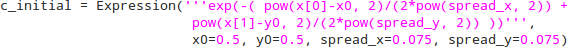
\includegraphics[width=0.75\columnwidth]{images/ufl_expression.png}
   \caption{An example of a UFL expression.}
   \label{fig:ufl_expression}
\end{figure}

\begin{figure}
   \centering
   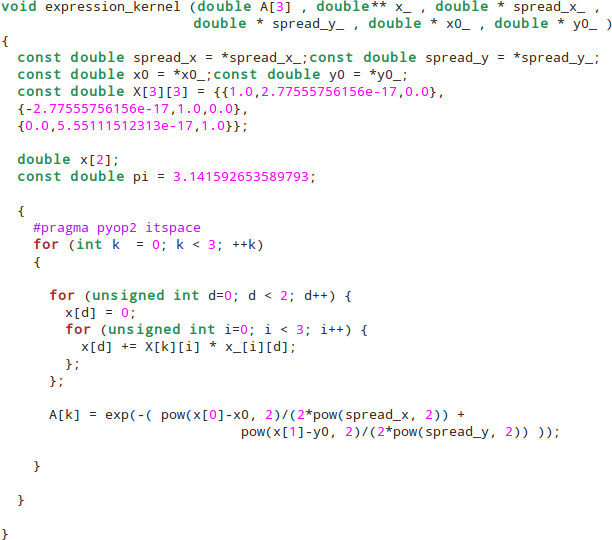
\includegraphics[width=0.75\columnwidth]{images/c_kernel.png}
   \caption{An example of C code, generated automatically, for the purpose of evaluating an expression defined by a high-level, near-mathematical UFL statement.}
   \label{fig:c_kernel}
\end{figure}

\section{Setup}
Before running the models in Firedrake-Fluids, please ensure that all the dependencies specified in the README file are satisfied.

Firedrake-Fluids comprises a collection of Python files containing the implementation of the different models; a set of schema files used to define the different options a simulation configuration file can take; and a set of test cases to help ensure the correctness of the models.


\chapter{Shallow water model}
The shallow water model solves the non-linear, non-rotational shallow water equations which describe the dynamics of a free surface and a depth-averaged velocity field. For modelling purposes, the free surface is split up into a mean component $H$ (i.e. the hydrostatic depth to the seabed) and a perturbation component $h$ (see Figure \ref{fig:shallow_water_setup}).

\begin{figure}
   \centering
   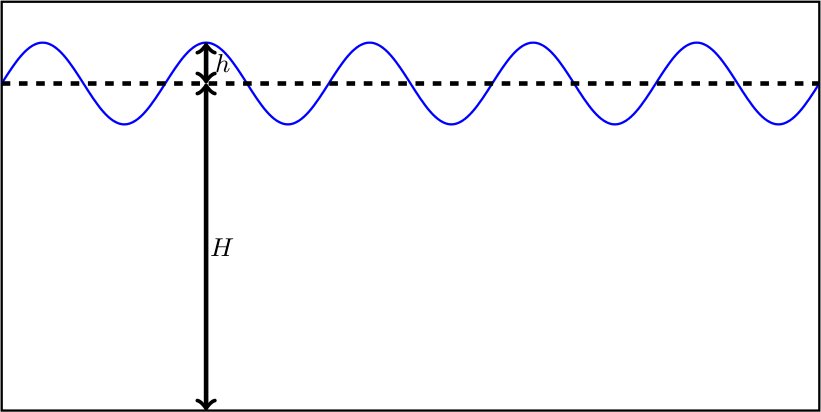
\includegraphics[width=0.6\columnwidth]{images/shallow_water_h_H.png}
   \caption{Single-layer shallow water set-up.}
   \label{fig:shallow_water_setup}
\end{figure}

\section{Model equations}
The shallow water equation set comprises a momentum equation and a continuity equation, each of which are defined below. These are defined on a domain $\Omega$ and for a time $t \in [0, T]$.

\subsection{Momentum equation}
The momentum equation is solved in non-conservative form such that
\begin{equation}
   \frac{\partial \mathbf{u}}{\partial t} + \mathbf{u}\cdot\nabla\mathbf{u} = -g\nabla h + \nabla\cdot\mathbb{T} - C_D\frac{||\mathbf{u}||\mathbf{u}}{(H + h)},
\end{equation}
where $g$ is the acceleration due to gravity, $\mathbf{u}$ is the velocity, and $C_D$ is the non-dimensional drag coefficient. The stress tensor $\mathbb{T}$ is given by 
\begin{equation}
   \mathbb{T} = \nu\left(\nabla\mathbf{u} + \nabla\mathbf{u}^{\mathrm{T}}\right) - \frac{2}{3}\nu\left(\nabla\cdot\mathbf{u}\right)\mathbb{I},
\end{equation}
where $\nu$ is the isotropic kinematic viscosity, and $\mathbb{I}$ is the identity tensor.

\subsection{Continuity equation}
The continuity equation is given by
\begin{equation}
   \frac{\partial h}{\partial t} + \nabla\cdot\left(\left(H + h\right)\mathbf{u}\right) = 0.
\end{equation}

\subsection{Discretisation}
The model equations are discretised using a Galerkin finite element method. Essentially, this begins by deriving the weak form of the equations by multiplying through by a test function $\mathbf{w} \in H^1(\Omega)^3$ (where $H^1(\Omega)^3$ is the first Hilbertian Sobolev space \citep{Elman_etal_2005}) and integrating over $\Omega$. In the case of the momentum equation, this becomes
\begin{eqnarray}
   \nonumber\int_{\Omega}\mathbf{w}\cdot\frac{\partial \mathbf{u}}{\partial t}\ \mathrm{dV} + \int_{\Omega}\mathbf{w}\cdot(\mathbf{u}\cdot\nabla\mathbf{u}) \ \mathrm{dV} = -\int_{\Omega}g\mathbf{w}\cdot\nabla h \ \mathrm{dV} + \int_{\Omega}\nabla\mathbf{w}\cdot \mathbb{T} \ \mathrm{dV} \\- \int_{\Omega}C_D\mathbf{w}\cdot\frac{||\mathbf{u}||\mathbf{u}}{(H + h)} \ \mathrm{dV}.
\end{eqnarray}
A solution $\mathbf{u} \in H^1(\Omega)^3$ is sought such that it is valid $\forall \mathbf{w} \in H^1(\Omega)^3$.

The solution fields $\mathbf{u}$ and $h$ are each represented by a set of interpolating basis functions, such that
\begin{equation}
   \mathbf{w} = \sum_{i=1}^{N_\mathrm{u\_nodes}} \phi_i\mathbf{w}_i,
\end{equation}
\begin{equation}
   \mathbf{u} = \sum_{i=1}^{N_\mathrm{u\_nodes}} \phi_i\mathbf{u}_i,
\end{equation}
and
\begin{equation}
   h = \sum_{i=1}^{N_\mathrm{h\_nodes}} \psi_ih_i,
\end{equation}
where $\phi_i$ and $\psi_i$ are the basis functions representing the velocity and free surface perturbation fields, respectively; $N_\mathrm{u\_nodes}$ and $N_\mathrm{h\_nodes}$ are the number of velocity and free surface solution nodes, respectively; and the coefficients $\mathbf{u}_i$ and $h_i$ are to be found by a solution method. If the basis functions $\phi_i$ are continuous across each cell/element in the mesh, then the method is known as a \textit{continuous} Galerkin (CG) method, whereas if the basis functions are discontinuous, then the method is known as a \textit{discontinuous} Galerkin (DG) method.

The momentum equation, discretised in space, then becomes a matrix system:
\begin{equation}
   \mathbf{M}\frac{\partial\mathbf{u}}{\partial t} + \mathbf{A}(\mathbf{u})\mathbf{u} + \mathbf{K}\mathbf{u} = -\mathbf{C}h + \mathbf{D}(\mathbf{u}, h)\mathbf{u},
\end{equation}
where $\mathbf{M}$, $\mathbf{A}$, $\mathbf{K}$, $\mathbf{C}$ and $\mathbf{D}$ are the mass, advection, stress, gradient and drag matrices, respectively.

The time-derivative is discretised using the implicit backward Euler method, yielding a fully discrete system of equations:
\begin{eqnarray}
   \mathbf{M}\frac{\mathbf{u}^{n+1} - \mathbf{u}^{n}}{\Delta t} + \mathbf{A}(\mathbf{u}^{n+1})\mathbf{u}^{n+1} + \mathbf{K}\mathbf{u}^{n+1} = -\mathbf{C}h^{n+1} + \mathbf{D}(\mathbf{u}^{n+1}, h^{n+1})\mathbf{u}^{n+1}.
\end{eqnarray}

The finite element method is also applied to the continuity equation, which must be solved along with the momentum equation, yielding a block-coupled system. In Firedrake-Fluids, this system is preconditioned using a fieldsplit preconditioner \citep{Brown_etal_2012} and solved with the GMRES linear solver \citep{SaadSchultz_1986}.

\section{Configuring a simulation}
The configuration/setup of a shallow water simulation in Firedrake-Fluids is defined in a Shallow Water Markup Language (.swml) file. This is essentially an XML file that contains tags/elements which are specific to the context of a shallow water simulation. The full range of possible options that are available to the user are defined by a set of schema files in the \texttt{schemas} directory; these can be thought of as `templates' from which an .swml setup file can be constructed.

Creating a shallow water setup/configuration file is best done using the Diamond graphical user interface (GUI) \citep{Ham_etal_2009} that is supplied with the libspud dependency. At the command line, from the Firedrake-Fluids base directory, creating an .swml file called \texttt{example.swml} can be done using

\texttt{diamond -s schemas/shallow\_water.rng example.swml}

Note that the -s flag is used to specify the location of the schema file \texttt{shallow\_water.rng}, while the final command line argument is the name of the setup file we want to create. The Diamond GUI will look something like the one shown in Figure \ref{fig:diamond}.

\begin{figure}[!ht]
   \centering
   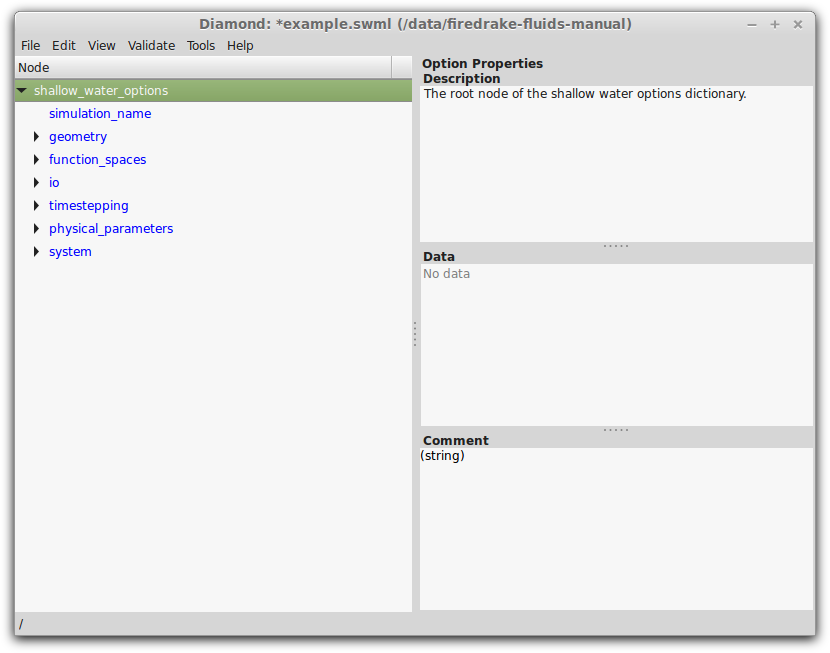
\includegraphics[width=1\columnwidth]{images/diamond.png}
   \caption{The Diamond \citep{Ham_etal_2009} graphical user interface. Notice that all the available options are currently in blue; this means that they still need to be specified the user, after which the font colour will turn black.}
   \label{fig:diamond}
\end{figure}

Details of each of the options (and sub-options underneath, displayed by clicking the black arrows) are given in the following sub-sections.

\subsection{Simulation name}
All simulations must be given a name under \texttt{/simulation\_name}. This name is used when outputting solution files created during the simulation. Please use alpha-numeric characters and avoid using non-standard characters such as ampersands, commas, semi-colons, etc here.

\subsection{Geometry}
The \texttt{/geometry} section of the setup file concerns the dimension of the problem, and the location of the computational mesh used to discretise the domain.

\subsection{Function spaces}

\subsection{Input/output (I/O)}

\subsection{Timestepping}

\subsection{Physical parameters}

\subsection{System: Core fields}
The model requires three fields to be set up under the \texttt{/system/core\_fields} section of the setup file. These are the key fields used in shallow water simulations, and are named
\begin{itemize}
   \item \textit{Velocity} (a prognostic field, corresponding to $\mathbf{u}$).
   \item \textit{FreeSurfacePerturbation} (a prognostic field, corresponding to $h$)
   \item \textit{FreeSurfaceMean} (a prescribed field, corresponding to $H$)
\end{itemize}
It is here that the initial and boundary conditions for the fields can be specified.

\subsubsection{Boundary conditions}
\begin{itemize}
   \item \textit{Dirichlet}: Strong Dirichlet boundary conditions can be enforced for both the FreeSurfacePerturbation and Velocity fields by selecting the \texttt{dirichlet} type.
   \item \textit{No-normal flow}: Imposing a no-normal flow condition for velocity can currently only be done weakly by integrating the continuity equation by parts and selecting the \texttt{no\_normal\_flow} boundary condition type in the configuration options.
   \item \textit{Flather}: A \cite{Flather_1976} open boundary condition can be imposed weakly by integrating the continuity equation by parts and selecting the \texttt{flather} boundary condition type in the configuration options. This boundary condition enforces:
   
   
   . Any difference between the exterior values and the simulated values along the boundary is allowed out of the domain in such a way that minimises spurious reflections.
\end{itemize}

\subsection{System: Equations}

\subsubsection{Spatial discretisation}
The spatial discretisation (continuous or discontinuous Galerkin) currently depends on the continuity of the function spaces in use, rather than on the choices made in this option. However, if \texttt{continuous\_galerkin} is selected, there are stabilisation-related sub-options available to stabilise the advection term when using CG. See Chapter \ref{chap:stabilisation} for more information on the stabilisation schemes available.

\subsubsection{Drag}
To include the quadratic drag term in the momentum equation, the \texttt{drag\_term} option must be enabled under \texttt{/system/equations/momentum\_equation/} and the non-dimensional drag coefficient $C_D$ should be specified.

 
\section{Running a simulation}

\section{Current limitations}
\begin{itemize}
   \item When using a discontinuous Galerkin method, the form of the stress tensor is currently restricted to:
   \begin{equation}
      \mathbb{T} = \nu\nabla\mathbf{u}.
   \end{equation}
   \item When using a discontinuous Galerkin discretisation, the interior penalty method is the only method available for determining the value of $\nabla\mathbf{u}$ at the discontinuous interior element boundaries. Similarly, only a simple upwinding method can be used to determine $\mathbf{u}$ at along interior element boundaries.
\end{itemize}

\chapter{Stabilisation methods}\label{chap:stabilisation}

\section{Streamline upwind}


%%%%%%%%%%%%%%%%%%%%%%%%%%%%%%%%%%%%%%%%%%%
%%%%%%% Turbulence parameterisation %%%%%%%
%%%%%%%%%%%%%%%%%%%%%%%%%%%%%%%%%%%%%%%%%%%
\chapter{Turbulence parameterisation}
This chapter describes the turbulence models that are available in Firedrake-Fluids.

\section{Large Eddy Simulation (LES)}

\subsection{Smagorinsky model}



%%%%%%%%%%%%%%%%%%%%%%%%%%%%%%%%%
%%%%%%% Diagnostic fields %%%%%%%
%%%%%%%%%%%%%%%%%%%%%%%%%%%%%%%%%
\chapter{Diagnostic fields}
Some stand-alone functions are available in the \texttt{diagnostics.py} file for computing flow diagnostics.

\section{Courant number}
The Courant number diagnostic computes the field defined by
\begin{equation}
   \frac{||\mathbf{u}||\Delta t}{\Delta x},
\end{equation}
where $\Delta t$ is the time-step size and $\Delta x$ is the element size (more specifically, it is twice the element's circumradius).

\section{Divergence}
This diagnostic field computes the divergence
\begin{equation}
   \nabla\cdot\mathbf{u},
\end{equation}
of a vector field $\mathbf{u}$.

\bibliographystyle{plainnat}
\bibliography{manual}

\end{document}
